\section{Introduction}

\begin{frame}{Motivation}

\begin{columns}
	\column{0.5\textwidth}
\begin{block}{The Context}
	A \textit{delegator} (verifier) requests a \textit{worker} (prover) to perform a computation for her.
\end{block}
\onslide<+->
\begin{itemize}[<+- | alert@+>]
	\item Large scale distributed computation (e.g. volunteer computation, SETI@home,\dots)
	\item Cloud computing.
	\item Weak peripheral devices.
\end{itemize}
\column{0.5\textwidth}
\begin{figure}
	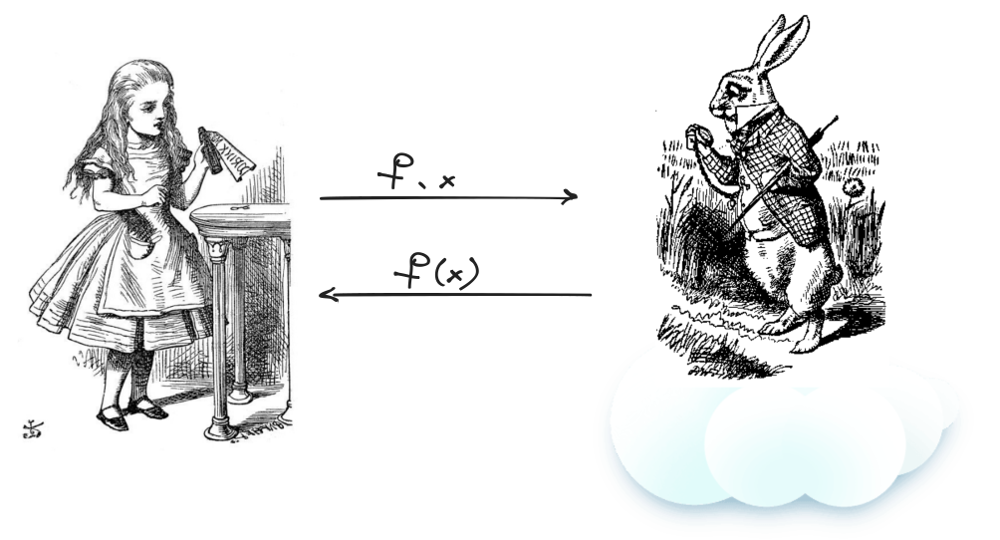
\includegraphics[scale=0.17]{pics/alice.png}
\end{figure}
\end{columns}
\pause
\bigskip
\textbf{Issue: } Untrusted Workers.\\
\pause
\medskip
\textbf{Verifiable Computation (VC):} Practical protocols offering guarantees in presence of untrusted workers.
\end{frame}

\begin{frame}[t]{Rational Verifiable Computation}
\textbf{Verifiable Computation (VC):} Practical protocols offering guarantees in presence of untrusted workers.\\ \pause
\vspace{1.6cm}
{\large \textbf{Our Focus: } VC where workers are \textbf{rational}, \pause i.e. maximizing \textit{incentives}.} \pause

\vspace{1.3cm}
\textbf{Why is this model interesting?}

%TODO: add context for rational provers
% TODO: Add picture 

\end{frame}


\begin{frame}[t]{Advantages of Exploiting Rationality}

Assuming a rational adversary (instead of an arbitrary one) clearly gives us a weaker model.\\\vspace{1cm}
\pause
\textbf{Yet, a rational model buys us:}
\begin{itemize}
	\item Efficient Protocols (especially verification);
	\item Simple Protocols;
	\item  Unconditional Results (often).
\end{itemize}

\end{frame}

\begin{frame}{Is this Model a Plausible Approximation?}
\begin{block}{Incentives in Outsourced Computation:}
	\begin{itemize}
		\item  payments for computations on the cloud; % XXX: who applies this model?
		\item 'rewarded' volunteer computation (SETI@HOME, GridCoin);
		\item  rewards for mining in cryptocurrencies.
	\end{itemize}
\end{block}
%\pause 
%\textbf{What are the Advantages?}
\end{frame}


% Metaphor

% TODO: Add next to each point a hint about the parts of the talk related to it.
\begin{frame}[t]{My Thesis, Succinctly}
	\textbf{Goal of Rational VC:} guarantees in presence of rational (and untrusted) workers.\\\vspace{0.9cm} \pause
	\textbf{This Talk:}\\
	\begin{enumerate}
		\item We can obtain such guarantees when delegating (subsets of) \textit{feasible} computations.\pause %This ``delegation'' is very efficient.\pause
		\item If a server ``cares'' about \textit{costs of computation}, existing techniques have a limitation (no multiple delegations); \pause I describe techniques without this flaw.\pause
		\item Alternative approach to solve (2) through minimal complexity assumptions:\pause  obtain protocols where \textit{cheating does cost more than acting honestly}.
	\end{enumerate}
\end{frame}

% Papers
\begin{frame}{Papers Related to This Thesis}
\begin{itemize}
	\item M. Campanelli, and R. Gennaro. ``Sequentially composable rational proofs." \textit{International Conference on Decision and Game Theory for Security. Springer, Cham, 2015.}
	\item M. Campanelli, and R. Gennaro. ``Efficient Rational Proofs for Space Bounded Computations." \textit{International Conference on Decision and Game Theory for Security. Springer, Cham, 2017.}
	\item M. Campanelli and R. Gennaro. ``Fine-Grained Secure Computation'' \textit{Submitted to TCC 2018}
\end{itemize}
\end{frame}


